\section{Analysis}
\label{sec:analysis}

For each of our six simulations, we use the 6-D phase space halo finder code \rockstar\ to identify spherical overdensity halos at each timestep.  \rockstar\ follows an adaptive hierarchical refinement of friends-of-friends halos in 6-D phase space\cn, allowing determination of halo properties such as constituent friends-of-friends particles, particles within the virial radius, halo mass, position, virial radius, internal energy, and substructure.  \rockstar\ claims to be able to track halos down to a threshold of around 20 particles\cn, but we use a more conservative 100 particle threshold for our analysis.  We use all particles found within the virial radius to define our halos and their properties.

We match halos between companion simulations with our \crossmatch\ code\cn.  Each pair of simulations is initialized with the same particle ID scheme, so that a given particle ID corresponds to the same particle in each simulation.  This allows us to match particle-to-particle between the simulations and identify matching halos based on the highest fraction of matching particles contained in each at any given timestep.  \textcolor{red}{Add sentence about ``best matching'' and existence of match in both directions.}  We find, for example, matches for about \textcolor{red}{xx\%} of halos above our particle count threshold at $z = 6$.  With halo catalogues matched between simulations, we can compare properties of individual corresponding halos.  We ``stack'' the three simulation boxes for each initialization method, and combine the halos from each into one larger sample in our analysis.

%\begin{figure}[h]
%	\centering
%	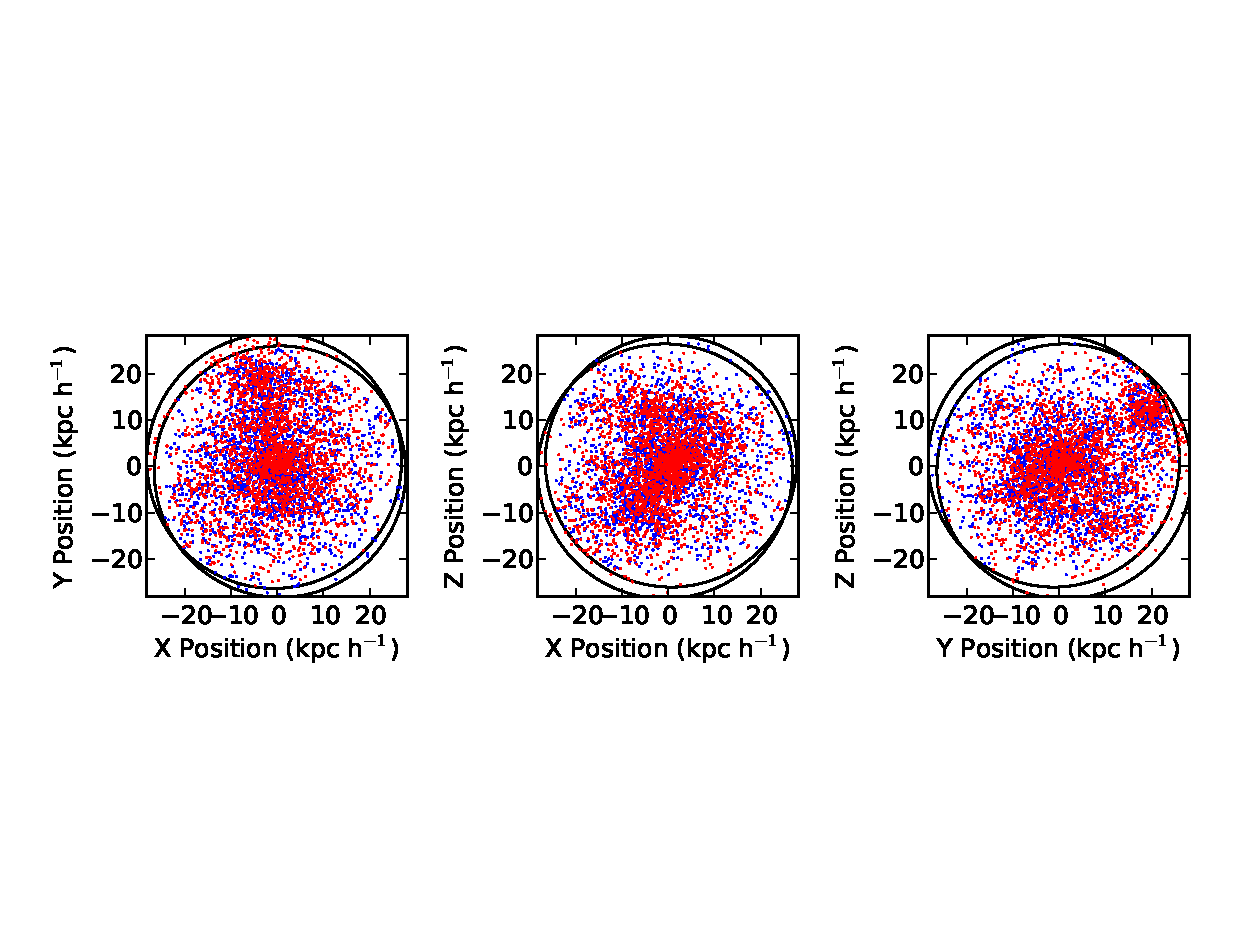
\includegraphics[width=3.0in]{match_particles.eps}
%	\caption{\footnotesize Projections of particle positions and virial radii for two matching halos in corresponding \lpt\ and \za\ simulations.  \lpt particles are shown in blue, and \za particles are shown in red.  The circles represent the virial radii for each halo.  \textcolor{red}{(Reduce size of bounding box.  All figures need bigger labels and thicker lines.)}}
%	\label{fig:match_particles}
%\end{figure}

Halo concentration $c=R_{vir}/R_{s}$ is derived from \rockstar's output for $R_{s}$ and $R_{vir}$, where $R_{s}$ is the scale radius defined by the NFW\cn\ profile
\begin{equation} \label{eq:nfw_profile}
	\rho(r) = \frac{ \rho_{0} }{ \frac{ r }{ R_{s}} \left( 1 + \frac{r}{R_{s}} \right)^{2} }
\end{equation}
and $R_{vir}$ is the virial radius as defined by \citet{1998ApJ...495...80B}.

To verify the accuracy of the \rockstar\ fit, we independently find density profiles for several halos and compare the fit parameters such as $R_{s}$.  For each halo, we fit an NFW density profile to logarithmic radial bins of particle position with a non-linear least squares fitting routine from the SciPy library.  From this, we measure the scale radius and, along with virial radii from \rockstar, the concentration.  The bottom two rows of Figure~\ref{fig:halo-pair}, for example, show the fitting results for a particle matched halo pair.  For halos fit by our method, our results are in relatively good agreement with \rockstar.  However, as we do not find an acceptable fit for every halo, we use the more complete \rockstar\ data for the final concentration measurements.

%\begin{figure}[t]
%	\centering
%	\includegraphics[width=\linewidth]{density_profile.eps}
%	\caption{\footnotesize Density profile for a large $z = 6$ halo.  Mass density is found in logarithmic radial bins from the simulation resolution limit to the virial radius of the halo.  The red curve is the resultant NFW profile fit.  The dot-dash line is the scale radius for the fit profile.  The top three panels are the projected density of the halo.  \textcolor{red}{(Change colormap to match other plots.)}}
%	\label{fig:density_profile}
%\end{figure}
